\documentclass[12pt,
               color={usenames,   % Since beamer loads color package 
                      dvipsnames},%  automatically \usepackage{color}   
                                  %  cannot be used to pass options.
%               draft,           % Draft WIP version without header &
                                %  footer. Faster compilation.
%               handout,         % Handout version. not sure what it does.
%               notes            % To print notes.
                    ]{beamer}   


%\includeonlyframes{SLIDENOW}    % Use when drafting for fast
                                % compile turnaround time.

%%%%%%%%%%%%%%%%%%%%%%%%%%%%%%%%%%%%%%%%%%%%%%%%%%%%%%%%%%%%%%%%%%%%%%%%%%%%%
% Theme customization

\usetheme[compress]{Ilmenau}    % Small circle based TOC on top bar
                                %  single line.
%\usetheme[width=1in]{Hannover}  % TOC left side bar.
%\usetheme{Szeged}               % Similar to Ilmenau except borders on
%                                %  top bar and bottom.
%\usecolortheme  {beetle}        % Grey and blue based.
\useinnertheme  {circles}       % Circle dingbats with no shading.
\usefonttheme[onlylarge]
                {structurebold} % Structure fonts are
                                % bold. Set to only the title / big
                                % fonts.
%\useoutertheme[compress,
%               footline=empty]
%               {miniframes}     % Don't use with explicit themes 

% Beamer elements customization: setbeamercolor/-font/-template
\setbeamercolor{title}                {fg=light3,bg=light1}
\setbeamercolor{subtitle}             {fg=dark1,bg=light1}
\setbeamercolor{date}                 {fg=dark1}
\setbeamercolor{institute}            {fg=dark1}
\setbeamercolor{frametitle}           {fg=dark1,bg=light1}
\setbeamercolor{framesubtitle}        {fg=light5}
\setbeamercolor{structure}            {fg=dark1}
\setbeamercolor{palette primary}      {fg=light1,bg=light2} % Palette
                                              % primary, secondary,
                                              % tertiary, quaternary
                                              % for headline and
                                              % footline 
\setbeamercolor{palette secondary}    {fg=dark2,bg=light3}
\setbeamercolor{palette tertiary}     {fg=light1,bg=light3} 
\setbeamercolor{palette quaternary}   {fg=light1,bg=light2} 
\setbeamercolor{normal text}          {fg=dark2,bg=light1} 
%\setbeamercolor{block body alerted}   {fg=white} %isn't working
\setbeamercolor{alerted text}         {fg=white} % contrast}  %light3} 
\setbeamercolor{block body}           {bg=light5}
\setbeamercolor{block title}          {fg=light1} %,bg=light3} % Uncomment 
                                              % for different block
                                              % heading background

% \setbeamertemplate{blocks}[rounded] % Blocks are rounded on the
%                                     % corners
\setbeamertemplate{blocks}[default] % Blocks are not rounded on the
                                    % corners

\setbeamerfont{framesubtitle}{series={\fontseries{c}}} % Condensed
                                %shape=\sc             % Small caps

%%%%%%%%%%%%%%%%%%%%%%%%%%%%%%%%%%%%%%%%%%%%%%%%%%%%%%%%%%%%%%%%%%%%%%%%%%%%%
% Packages used
\usepackage{../lib/mylatexlib}


\usepackage{setspace}
\usepackage{latexsym}
\usepackage{amssymb}
\usepackage{amsfonts}
\usepackage{amsmath}
%\usepackage{epsfig}
%\usepackage{graphicx}
%\usepackage{epstopdf}
\usepackage{algorithm}
\usepackage{algorithmic}
\usepackage{enumerate}
\usepackage[normalem]{ulem}  % Underline. normalem keeps the default
                             % \em to be italics. 
\usepackage{textcomp}
%\usepackage{pifont}
%\usepackage{natbib}
%\usepackage[finalnew]{../lib/trackchanges}


%%%%%%%%%%%%%%%%%%%%%%%%%%%%%%%%%%%%%%%%%%%%%%%%%%%%%%%%%%%%%%%%%%%%%%%%%%%%%
% Loading spcial fonts
\DeclareMathAlphabet{\mathpzc}{OT1}{pzc}{m}{it}
\DeclareMathAlphabet{\mathcalligra}{T1}{calligra}{m}{n}


%%%%%%%%%%%%%%%%%%%%%%%%%%%%%%%%%%%%%%%%%%%%%%%%%%%%%%%%%%%%%%%%%%%%%%%%%%%%%
% Color definitions

%% Inspired by Kuler - Vintage Beach Wear -
%% http://kuler.adobe.com/#themeID/1507195 
\definecolor{dark1}      {HTML}{8A866A}   % Goldish gray     
                                          %     [Structure, Block heading]
\definecolor{light1}     {HTML}{FFF0C2}   % Pale amber          
                                          %     [Slide BG] 
\definecolor{light2}     {HTML}{9C968B}     % Gambogeish gray [???]
\definecolor{light3}     {HTML}{A36D5C}   % Grayish vermilion   
                                          %     [Title, Header & footer BG] 
\definecolor{dark2}      {HTML}{473C35}   % Dark grayish tangelo
                                          %     [Slide normal text FG]
\definecolor{light5}     {HTML}{A8A87D}   % Greyish olive
                                          %     [Block BG]
\definecolor{contrast}   {HTML}{197DE5}   % Brilliant azure     
                                          %     [Stark Contrast]



%%%%%%%%%%%%%%%%%%%%%%%%%%%%%%%%%%%%%%%%%%%%%%%%%%%%%%%%%%%%%%%%%%%%%%%%%%%%%
% String defs
\def\cA{{\cal A}}  \def\cB{{\cal B}}  \def\cC{{\cal C}}  \def\cD{{\cal D}}
\def\cE{{\cal E}}  \def\cF{{\cal F}}  \def\cG{{\cal G}}  \def\cH{{\cal H}}
\def\cI{{\cal I}}  \def\cJ{{\cal J}}  \def\cK{{\cal K}}  \def\cL{{\cal L}}
\def\cM{{\cal M}}  \def\cN{{\cal N}}  \def\cO{{\cal O}}  \def\cP{{\cal P}}  
\def\cQ{{\cal Q}}  \def\cR{{\cal R}}  \def\cS{{\cal S}}  \def\cT{{\cal T}}  
\def\cU{{\cal U}}  \def\cV{{\cal V}}  \def\cW{{\cal W}}  \def\cX{{\cal X}}
\def\cY{{\cal Y}}  \def\cZ{{\cal Z}}  \def\hA{{\hat A}}  \def\hB{{\hat B}}
\def\hC{{\hat C}}  \def\hD{{\hat D}}  \def\hE{{\hat E}}  \def\hF{{\hat F}}
\def\hG{{\hat G}}  \def\hH{{\hat H}}  \def\hI{{\hat I}}  \def\hJ{{\hat J}}
\def\hK{{\hat K}}  \def\hL{{\hat L}}  \def\hP{{\hat P}}  \def\hQ{{\hat Q}}
\def\hR{{\hat R}}  \def\hS{{\hat S}}  \def\hT{{\hat T}}  \def\hX{{\hat X}}
\def\hY{{\hat Y}}  \def\hZ{{\hat Z}}
\def\A{{\mathcal A}}  \def\bI {\mathbb I}
\def\C{{\mathcal C}}  \def\bO {\mathbb O}
\def\F{{\mathcal F}}  \def\cl {\mathpzc{l}}
\def\H{{\mathcal H}}  \def\cg {\mathpzc{g}}
                      \def\ccT{\mathpzc{T}}

\def\overlap   {\between}
\def\eps       {\epsilon}
\def\icppl     {\maltese} 
\def\invb      {\textreferencemark}
\def\assign    {\leftarrow}

\def\lndisplay      {1}
\def\commentboxsize {7cm}
\def\prelimspace    {2mm}
\def\alertseccolor {contrast}

% For BibTeX formatting \newblock
\def\newblock{\hskip .11em plus .33em minus .07em}
% for Natbib
%\bibpunct{(}{)}{;}{a}{,}{,}


%%%%%%%%%%%%%%%%%%%%%%%%%%%%%%%%%%%%%%%%%%%%%%%%%%%%%%%%%%%%%%%%%%%%%%%%%%%%%
% New/renew commands
% Format of comments in algorithmic package
\renewcommand{\algorithmiccomment}[1]
{ 
  \vspace {0.5mm}
  \hfill
  {\small
  \begin{tabular}{|r}
    \parbox[right]{\commentboxsize}{ \space \tt{ #1 }}\\  
    % {\tt /* #1 */} \hspace{2mm}
  \end{tabular}
  }
}


% % Theorems etc. 
% \newtheorem{observation}{Observation}
%%% 1 DEC
% \newcommand{\seq}[1]{\left\langle #1 \right\rangle}
% \newcommand{\set}[1]{\left\{ #1\right\}}
% \newcommand{\supp}[1]{supp\left( #1 \right)}
%%% END 1 DEC

%%%%%%%%%%%%%%%%%%%%%%%%%%%%%%%%%%%%%%%%%%%%%%%%%%%%%%%%%%%%%%%%%%%%%%%%%%%%%
% Title slide details
\title[{\bf tree path labeling} -- a generalization of consecutive
       ones property of binary matrices]
         {Tree Path Labeling of Set Systems}
\subtitle{A Generalization of Consecutive Ones Property}

\author[anju s $|$ \tt{anjuzabil@gmail.com}]{Anju Srinivasan}

\institute[CS09S012]
         {as part of {\bf M.\;S.} by Research \\ 
          advised by {\bf Dr.\;N.\;S.\;Narayanaswamy}\\ 
          CSE, IITM, Chennai - 36}

\date{18 Oct 2011}


%%%%%%%%%%%%%%%%%%%%%%%%%%%%%%%%%%%%%%%%%%%%%%%%%%%%%%%%%%%%%%%%%%%%%%%%%%%%%
% Document begins

\begin{document}

\frame{
  \titlepage
}

%\section*{Outline}
\frame[label=SLIDENOW]{
  \tableofcontents % [pausesections]
}


\section{Introduction}
\subsection{An Illustration}

\frame{
  \frametitle{An Illustration}

  \begin{centering}
  {\bf Caveat}
  \begin{itemize}
    \item A very simplistic example.
    \item Aims only to introduce the combinatorial problem of TPL.
  \end{itemize}
    
  \end{centering}
}

\frame{
  \frametitle{A Study Group Housing problem}
% \begin{centering}
  \begin{itemize}[<uncover@+->]
  \item A set of $n$ students arrive for a summer course, say
    $\{a,b,c,d,e,f,g,h,i,j,k\}$, $n= 11$.
  \item They form $m$ study groups, say $\{\textcolor{red}{R},
    \textcolor{blue}{B}, \textcolor{orange}{O},
    \textcolor{green}{G}\}$, $m = 4$
  \item A student may be in more than one study group but {\bf will} be in
    at least one, say
    \begin{itemize}
    \item $\textcolor{red}{R = \{g, h, i, j, k\}}$
    \item $\textcolor{blue}{B = \{a, b, e, g\}}$
    \item $\textcolor{orange}{O = \{c, b, d\}}$
    \item $\textcolor{green}{G = \{e, f , g, i\}}$
    \end{itemize}

  \item There are $n$ single occupancy apartments in the university campus for their accommodation.
  \item All these apartments are placed such that streets connecting
    them do not form loops
  \end{itemize}

\note{}  
%  \end{centering}
}

\frame{
  \frametitle{A Study Group Housing problem}
% \begin{centering}
  \begin{block}{The problem}
    {How should the students be allocated apartments such that
    each study group has the least distance to travel for a discussion?}
  \end{block}
%  \end{centering}
}


\frame{
  \frametitle{A Study Group Housing problem}
% \begin{centering}
   \only<1>{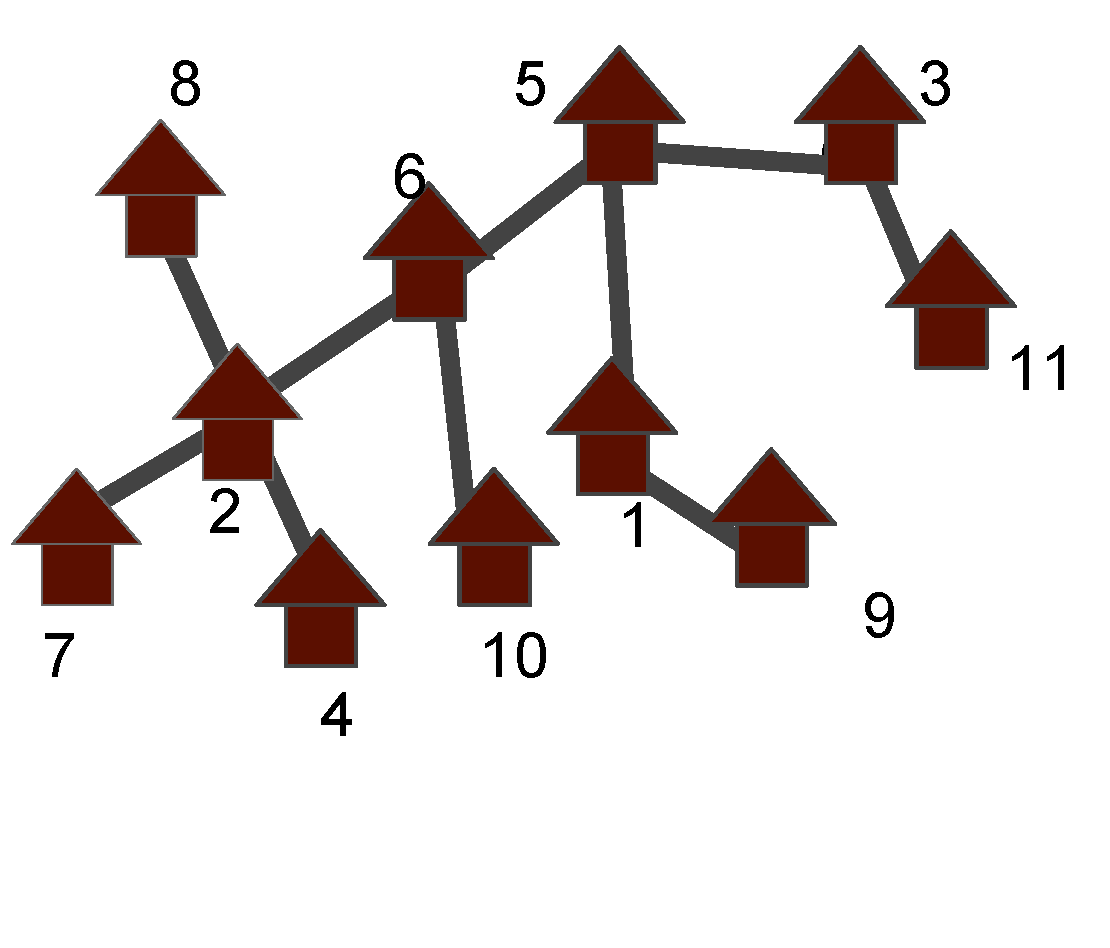
\includegraphics[scale=0.4]{a1.pdf}}
   \only<2>{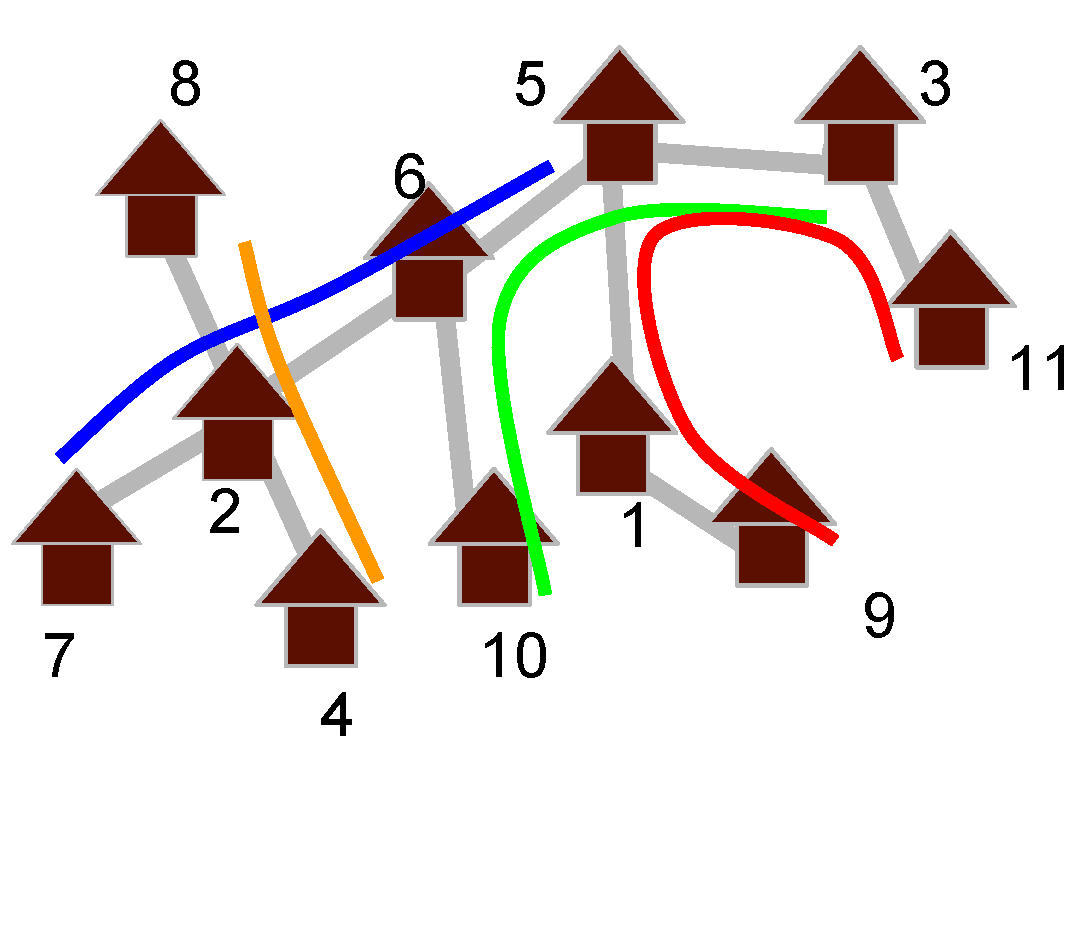
\includegraphics[scale=0.4]{a2.pdf}}
   \only<3>{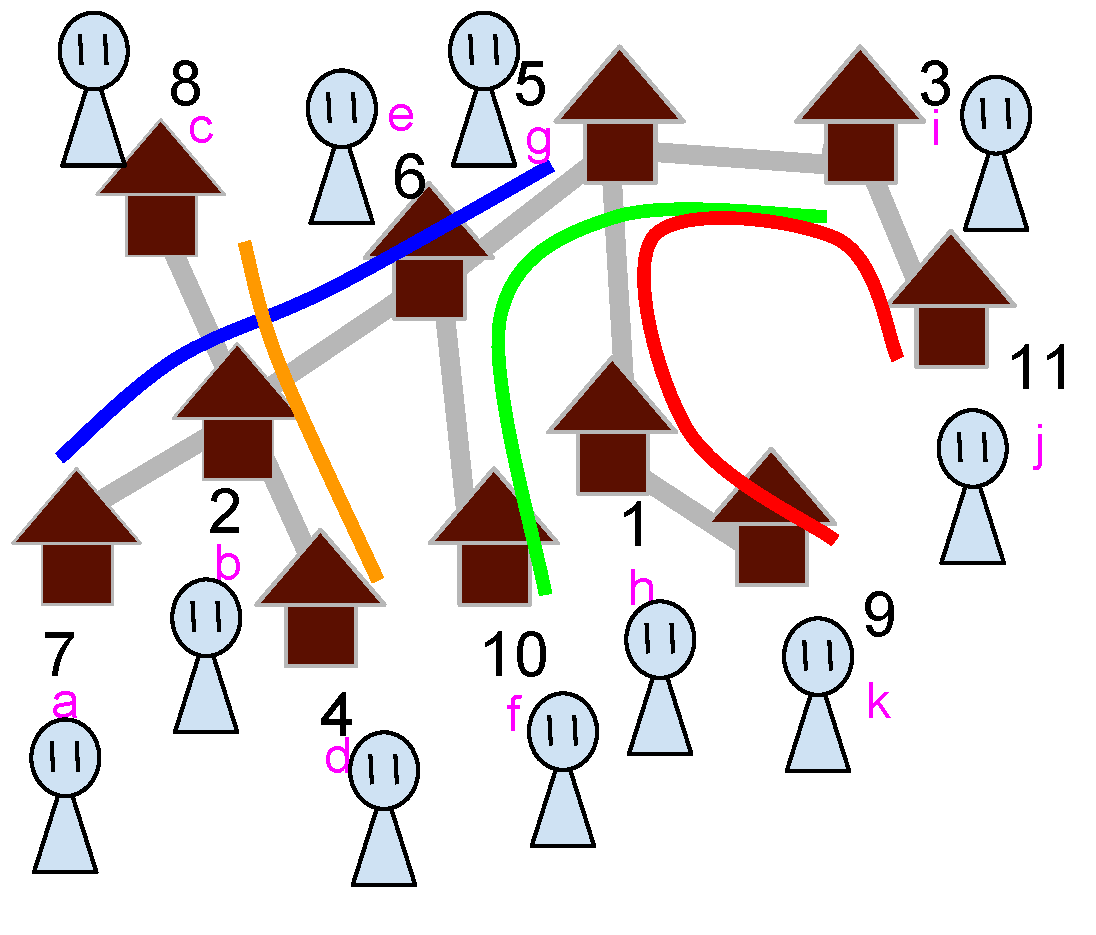
\includegraphics[scale=0.4]{a3.pdf}}
%  \end{centering}
}


\frame<1-5>{ \frametitle{Tree Path Labeling of Set Systems}
  \framesubtitle{The combinatorial problem terminology}

  \begin{block}{Terminology}

    \begin{itemize}
    \item The set of study groups i.e. sets of students $\rightarrow$
      \alert<2->{\sc Set system / Hypergraph}
    \item The streets with apartments $\rightarrow$ \alert<3->{\sc
        Target tree}
    \item The route mapping to study groups $\rightarrow$
      \alert<4->{\sc Tree Path Labeling (TPL)}
    \item The apartment allocation $\rightarrow$ \alert<5>{\sc Path
        Hypergraph Isomorphism}
    \end{itemize}
  \end{block}
}

\def\overlayht{4cm}

\frame<1-6>{
  \frametitle{Tree Path Labeling of Set Systems}
  \framesubtitle{The combinatorial problem} 

  \begin{block}{Terminology [contd.]}
    \begin{overlayarea}{\textwidth}{\overlayht} 
      \only<1>{There {\em exists} an apartment allocation that
          ``fits'' the route mapping }
      \only<2->{There {\em exists} a
          \alert<2->{hypergraph isomorphism} that ``fits'' the
          \alert<2->{TPL}\\}
      \only<3->{$\rightarrow$ the TPL is \alert<3->{\sc feasible}\\}

      \only<4->{There {\em exists} \only<4>{an apartment
          allocation}\only<5->{\alert<5-> {a hypergraph isomorphism}} that
          gives \only<4>{the optimal route mapping}
      \only<5->{\alert<5->{paths/adjacent vertices in tree}\\}} 
%       \only<4>{There {\em exists} an apartment allocation that
%       gives the optimal route mapping}
%       \only<5-> {There {\em exists} a
%       \alert<5->{hypergraph isomorphism} that gives 
%       \alert<5->{paths/adjacent vertices in tree}\\}
      \only<6->{$\rightarrow$ the hypergraph is a \alert<6->{\sc
       path hypergraph}}
      \end{overlayarea}
  \end{block}

}

\subsection{Motivation}
\frame{
  \frametitle{Consecutive Ones $\rightarrow$ Path Labeling}
  \framesubtitle{The motivation}

   \only<1>{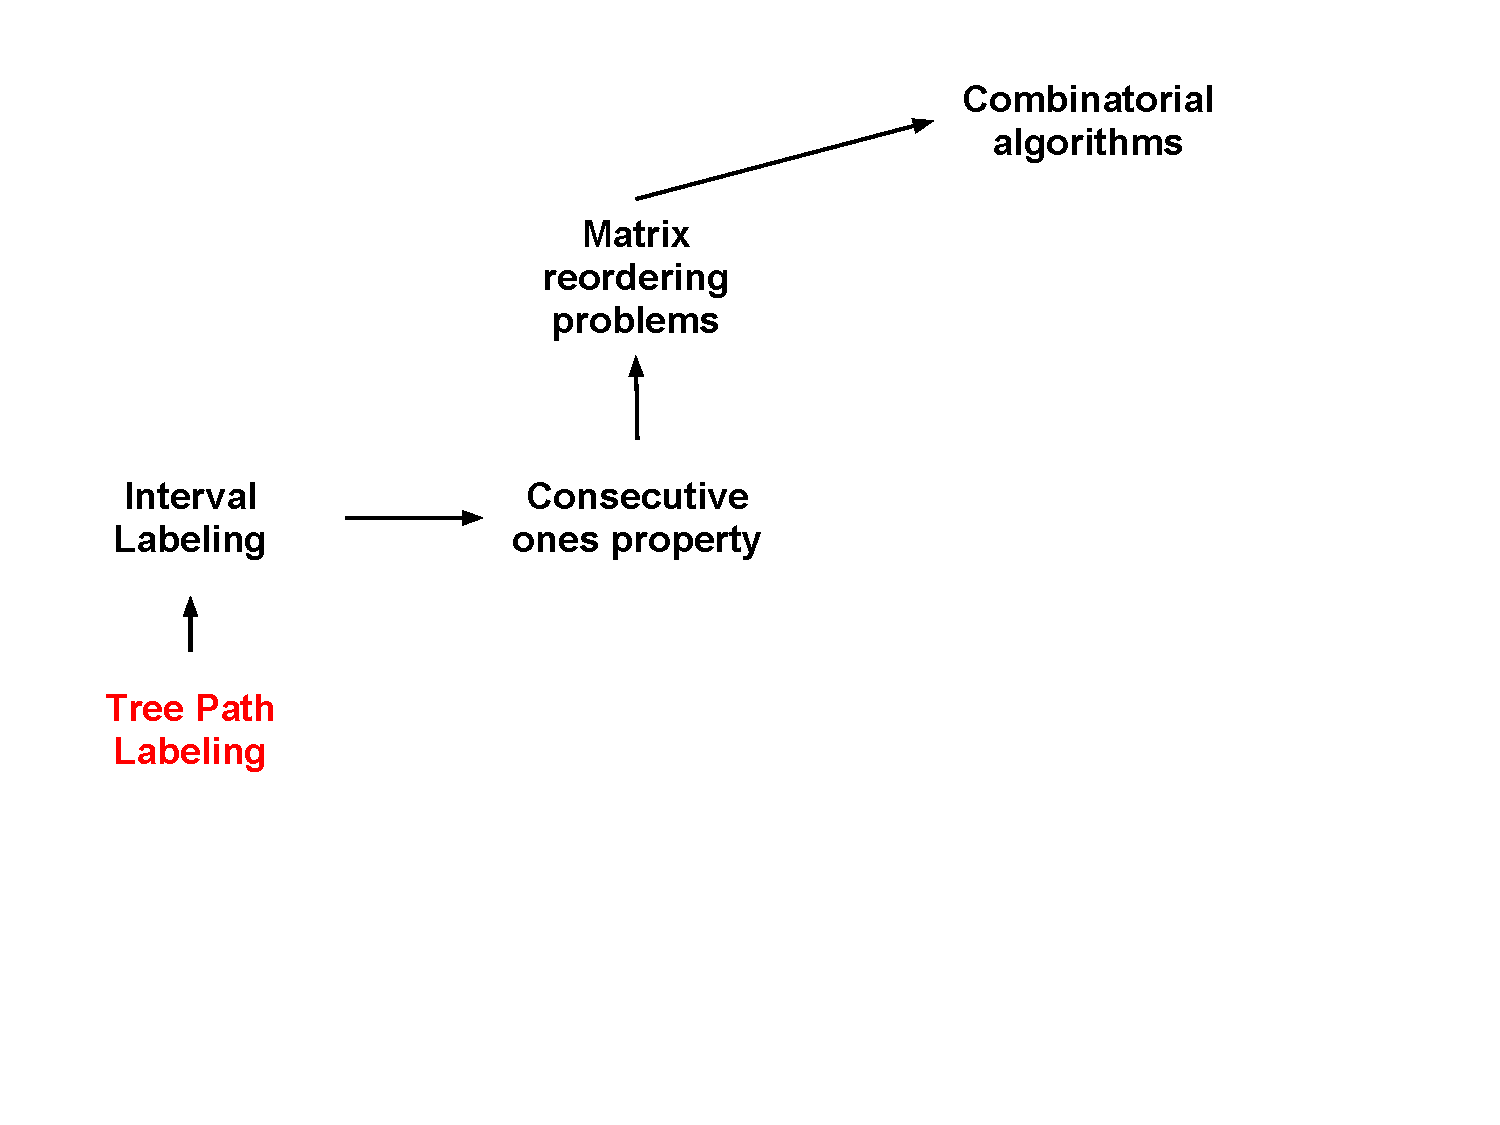
\includegraphics[scale=0.4]{m1.pdf}} 
  
  \tnote[a]{break it down into overlays}
  \note{}
}

\subsection{Definitions}

\frame{
  \frametitle{Tree path labeling of path hypergraphs}
  \framesubtitle{The two problems}
  
  \note<1>{}
  
  \begin{block}{1}
    {\alert<2>{Characterization} of a {\em feasible TPL} and finding
      the certificate for feasibility i.e. {\em hypergraph
        isomorphism}}
  \end{block}
  \note[item]<2>{Characterization -- hypergraph + target tree + TPL\\ 
      (1) is it feasible? \\
      (2)what is the isomorphism?}

  \begin{block}{2}
    {\alert<2>{Computation} of a {\em feasible TPL} if any}
  \end{block}
  \note[item]<2>{Computation -- hypergraph + target tree\\ 
      (1) does there exist a
      feasible TPL?

  }
}

\frame<1>[label=intro:q1]{
%\frame<1,9>[label=intro:q1]{
% 1   : display normal
% 9   : TBD defined prelim
% 2-7 : each TBD definition highlight
% 8   : misc definition highlight
  \begin{center}
    {\Huge 1}
  \end{center}
    \begin{block}{Characterization of feasible TPL}
    Given
    \begin{enumerate}[i. ]
    \item a \textcolor<9>{\alertseccolor}
           {\alert<2>{set system or hypergraph}} $\cF$,
    \item a \textcolor<9>{\alertseccolor}
           {\alert<3>{feasible} \alert<4>{TPL}} $\cl:\cF \rightarrow
      \cP$ where $\cP$ is a path system from tree $T$ and $
      \textcolor<9>{\alertseccolor}{\alert<5,2>{supp(} \cP \alert<5,2>{)}} = V(T)$,
    \end{enumerate}
    \uline{what is the \textcolor<9>{\alertseccolor}{\alert<6>{hypergraph
        isomorphism}}} \[\underline{\phi: \supp{\cF} \rightarrow
      \supp{\cP}}\] \uline{such that the
      \textcolor<9>{\alertseccolor}{\alert<7,4>{induced labeling}}} 
    $\underline{\cl_\phi = \cl}$?
  \end{block}

  \note[item]<1>{}
  \note[item]<9>{to understand this these will be defined in the
    following slides}
  \note[item]<2>{first we'll see what a set system or hypergraph is}
  \note[item]<6>{Next is hypergraph iso}
  \note[item]<4>{tree path labeling}
  \note[item]<3>{feasibility of TPL}
}

% \againframe<2>{intro:q1}

% \frame<1-3>{
%   \frametitle{}
%   \begin{definition}[Set system, Support of set system] 
%    The set $\F \subseteq (2^{U} \setminus
% \emptyset)$ is a \alert {set system} of a universe $U$ with $|U| = n$.\\

%    The \alert {support of a set system} $\F$ is
%     the union of all the sets in $\F$.\\ 
%    $ \ \ \ \ \ \ \ \ \ \ \ \ \ \ \alert{supp(\F) = \bigcup_{S \in \F}S}$
%   \end{definition}

%   \note[item]<1>{}

%   \begin{definition}<2->[Hypergraph] 
%   A \alert{hypergraph} is exactly same as a graph except that an
%   ``edge'' can have more than two
%   vertices and are called \alert{hyperedges}.
%   \end{definition}

%   \note[item]<2>{}

% %  \begin{block}<3>{} 
% %   $\cF$ can be \alert<3>{ visualized as a
% %       hypergraph} -- \alert<3>{ vertex set is $supp(\cF)$}, \alert<3>{ hyperedges are the sets
% %       in $\cF$.}
% % \end{block}

%   \only<3>{ 
%   $\cF$ can be \textbf{visualized as a
%       hypergraph} -- \textbf{vertex set is $supp(\cF)$},
%     \textbf{hyperedges are the sets 
%       in $\cF$.}
%    }

%   \note[item]<3>{}

% %   \begin{block}{Definition}
    
% %   \end{block}
% }

% \againframe<6>{intro:q1}

% \frame{
%   % \frametitle{}
%   \begin{definition}<1->[Hypergraph isomorphism \cite{kklv10}]
  
%     Two hypergraphs $\cF'$, $\cF''$ are said to be isomorphic,
%       \alert{ $\cF' \cong \cF''$}

%   $\ \ \ \ \ \ \ \ \ \ \ \ \ \ \ \ \ \ \ \ \ \ \ \ \ \ \ \ \ \ \ \ \ \
%   \Longleftrightarrow$        
 
%   there \alert{ exists a 
%     bijection $\phi: supp(\cF') \rightarrow supp(\cF'')$} s.t. \\

%     \alert{   for
%     all sets $A \subseteq supp(\cF')$
% $A \in \cF'$ $\Leftrightarrow$
%     $B \in \cF''$ where $B = \{\phi(x) \mid x \in
%     A\}$}, written as $B=\phi(A)$.
%   \end{definition}
% }

% \againframe<4>{intro:q1}

% \frame{
% %  \frametitle{Tree path labeling (TPL)}

%   \begin{overlayarea}{\textwidth}{5cm}
%   \begin{definition}<1->[Tree Path Labeling (TPL)]
%     For a set system $\cF$, \alert{$\cl: supp(\cF) \rightarrow \cP$} where
%     $\cP$ is a set of paths from $T$, is called a \alert{TPL} if their
%     intersection graphs are isomorphic \textcolor<2->{contrast}{(not
%       hypergraph isomorphism)} \alert{$\bI(\cF) \cong \bI(\cP)$},
%     $\cl$ is the isomorphism.\\
 
%    Alternate notation for the \alert{path representation} $\cP$ is \alert{$\cF^\cl$}.
%   \end{definition}
%   \only<2>{i.e. intersection properties are preserved. but {\bf not}
%     necessarily intersection cardinality properties.}
%   \end{overlayarea}
%   \begin{definition}<3->[Induced TPL]
%    If $\cF \cong \cP$ \textcolor<4>{contrast}{(hypergraph
%      isomorphism)} and $\phi$ is the isomorphism $\Longrightarrow$
%    this induces a path labeling. This is called \alert{induced path
%      labeling, $\cl_\phi$}
    
%   \end{definition}

% }

% \againframe<3>{intro:q1}

% \frame{
% %  \frametitle{Feasible labeling}

%   \begin{definition} [Feasible TPL]
%     A TPL $(\cF, \cl)$ is defined to be \alert{feasible} if
% % $\cF \cong \cF^\cl$ and this
% there is \alert{a hypergraph isomorphism $\phi: supp(\cF) \rightarrow
% supp(\cF^\cl)$} $=V(T)$ which induces path labeling $\cl_\phi: \cF \rightarrow
% \cF^\cl$ such that \alert{$\cl_\phi = \cl$}.
%   \end{definition}

%   \only<2->{ Recall:
%     \begin{itemize}
%     \item<2-> $\cF \cong \cF^\cl$ and $\phi$ is the \textbf{hypergraph
%         isomorphism}
%     \item<3-> $\bI(\cF) \cong \bI(\cF^\cl)$ and $\cl$ is the \textbf
%       {graph isomorphism}
%     \item<4-> \textbf{and} the induced TPL $\cl_\phi$ must be same as $\cl$.
%     \item<5-> If there is such a $\phi$ then $\cl$ is feasible.
%     \end{itemize}
%   }

% }

\frame<1>[label=intro:q2]{
%\frame<1-2>[label=intro:q2]{
  \begin{center}
    {\Huge {\tt 2}}
  \end{center}
  \begin{block}{Computing a feasible TPL}
    Given hypergraph $\cF$ with certain properties and a
    \alert<2>{$k$-subdivided star} $T$, \uline{can we find a feasible TPL 
      $\cl$ to $T$?}
  \end{block}
  \note{}
}

% \frame {
% %  \frametitle{$k$-subdivided star}

%   \begin{definition}[$k$-subdivided star]
%     A \alert{$k$-subdivided star} is a star with all its edges
%     subdivided exactly $k$ times.
%   \end{definition}

%   \only<2>{ 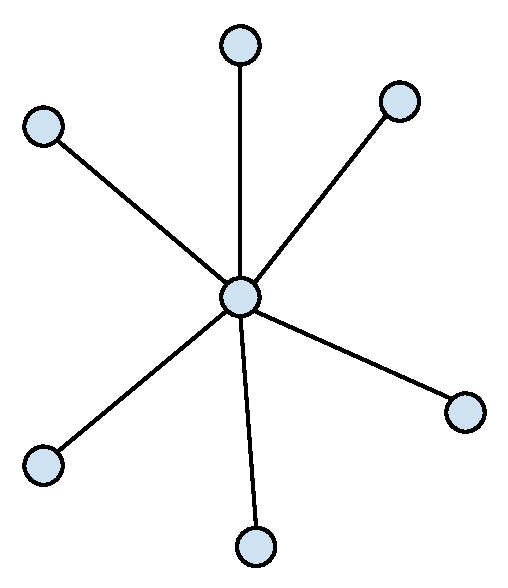
\includegraphics[scale=0.5]{star.pdf} $k = 0$ }
%   \only<3>{ 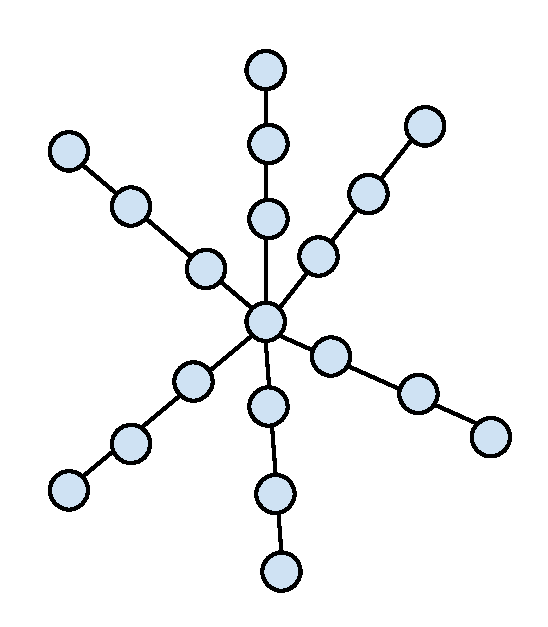
\includegraphics[scale=0.5]{kstar.pdf}  $k = 2$}

%   \note{we'll see details later.}
% }

% %\againframe<1>{intro:q2}


\section[Characterization]{Characterization of a feasible TPL}

\frame {
% \againframe<1>{intro:q1}
%   \note{recall this problem. we'll see the algorithms.}
  \begin{center}
    {\Huge 1}
  \end{center}
    \begin{block}{Characterization of feasible TPL}
    \end{block}
}



\subsection{ICPPL}
\frame [label=icppl:pr]{ %[label=SLIDENOW]{ % 
  \frametitle{ICPPL - a TPL with special properties}
  \framesubtitle{Intersection Cardinality Preserving Path Labeling}

  \tnote[a]{TBD list ICPPL properties}
  \note{}
}

\frame<1> [label=th:icpplth]{ % [label=SLIDENOW]{ % 
  \frametitle{The characterization}
  \framesubtitle{ICPPL + a filtering algorithm}

  \tnote[a]{TBD Write the theorem}
  \note{}
}

\subsection{Filtering algorithm}
\frame [label=flow:filtering]{ %[label=SLIDENOW]{ %
  \frametitle{The filtering algorithm}
  \framesubtitle{{\tt filter\_1}\\ 
                 {\tt filter\_2}\\ 
                 Algorithm {\tt get-hypergraph-isomorphism}}

  \tnote[a]{TBD flow chart of the filtering algorithm. see notes.}
  \note{}
}

\frame [label=al:filter1]{ %[label=SLIDENOW]{ %
  \frametitle{\tt filter\_1}
  \framesubtitle{Make leaves unique to paths} 

  \tnote[a]{TBD present the algorithm with images? with psuedocode on
    the side? f yeah. like dessert. apple pie with cream on the side please.}
  \note{}
}

\frame [label=al:filter2]{ %[label=SLIDENOW]{ %
  \frametitle{\tt filter\_2}
  \framesubtitle{Find elements that map to leaves}

  \tnote[a]{TBD present the algorithm with images? with psuedocode on
    the side? f yeah. like dessert. apple pie with cream on the side
    please.} 
  \note{}
}

\frame [label=al:treeprune]{ %[label=SLIDENOW]{ %
  \frametitle{Algorithm {\tt get-hypergraph-isomorphism}}
  \framesubtitle{Find hypergraph isomorphism $\phi$ - recursively use
    {\tt filter\_1} {\tt filter\_2}}

  \tnote[a]{TBD present the algorithm with images? with psuedocode on
    the side? f yeah. like dessert. apple pie with cream on the side
    please.} 
  \note{}
}

\againframe<1>{th:icpplth}     % Show theorem again before proof.
  \note{}

% \subsection{Proof and analysis}

% %\frame [label=SLIDENOW]{
% \frame [label=char:proof]{ 
%   \frametitle{Proof}
%  \framesubtitle{Outline}

%   \tnote[a]{Give outline of the proof.}
%   \note{}
% }

% %\frame [label=SLIDENOW]{
% \frame [label=char:proof]{ 
%   \frametitle{Brief analysis}
% %  \framesubtitle{Outline}

%   \tnote[a]{Give brief analysis.}
%   \note{}
% }


\section[Computation of TPL]{Computing a feasible TPL on
  $k$-subdivided trees} 

\againframe<1>{intro:q2}       % Show q2 again - refresher.
  \note{}

\subsection{Algorithm}

% \frame [label=SLIDENOW]{
\frame{ \frametitle{Special case} \framesubtitle{Interval assignment
    problem / COP}

  \begin{enumerate}
  \item<1-> $T$ is a path $\Longrightarrow$ paths in $T$ are intervals
    \tnote[a]{quick illustration}
  \item<1-> Only pairwise intersection cardinality needs to be
    preserved $\Longrightarrow$ ICPIA \cite{nsnrs09}
  \item<1-> Higher level intersection cardinalities preserved by {\bf
      Helly Property} -- \cite{mcg04}
  \item<1-> {\em filter\_1},{\em filter\_2} do not need the the {\bf
      exit} conditions. \tnote[a]{is this cryptic?}
  \end{enumerate}
  
  \begin{block}{}
    This problem is equivalent to Consecutive Ones Property of binary
    matrices \cite{nsnrs09}
  \end{block}

  \note{} }



% %\frame [label=TEST BIBTEX]{
% \frame {
%   \frametitle{???}
%   \cite{d08phd}\\
%   \cite{bl76}\\
%   \cite{fg65}
% }


% \subsection{Proof and analysis}

% \frame [label=SLIDENOW]{ 
%   \frametitle{Proof}
%   \framesubtitle{Outline}

%   \tnote[a]{Give outline of the proof.}
%   \note{}
% }

% \frame [label=SLIDENOW]{ 
%   \frametitle{Brief analysis}
% %  \framesubtitle{Outline}

%   \tnote[a]{Give brief analysis.}
%   \note{}
% }



\section{Conclusion}
\subsection{Application}
\frame
{
    \frametitle{Path Labeling $\rightarrow$  Graph Isomorphism}
    \framesubtitle{Application} 

   \only<1>{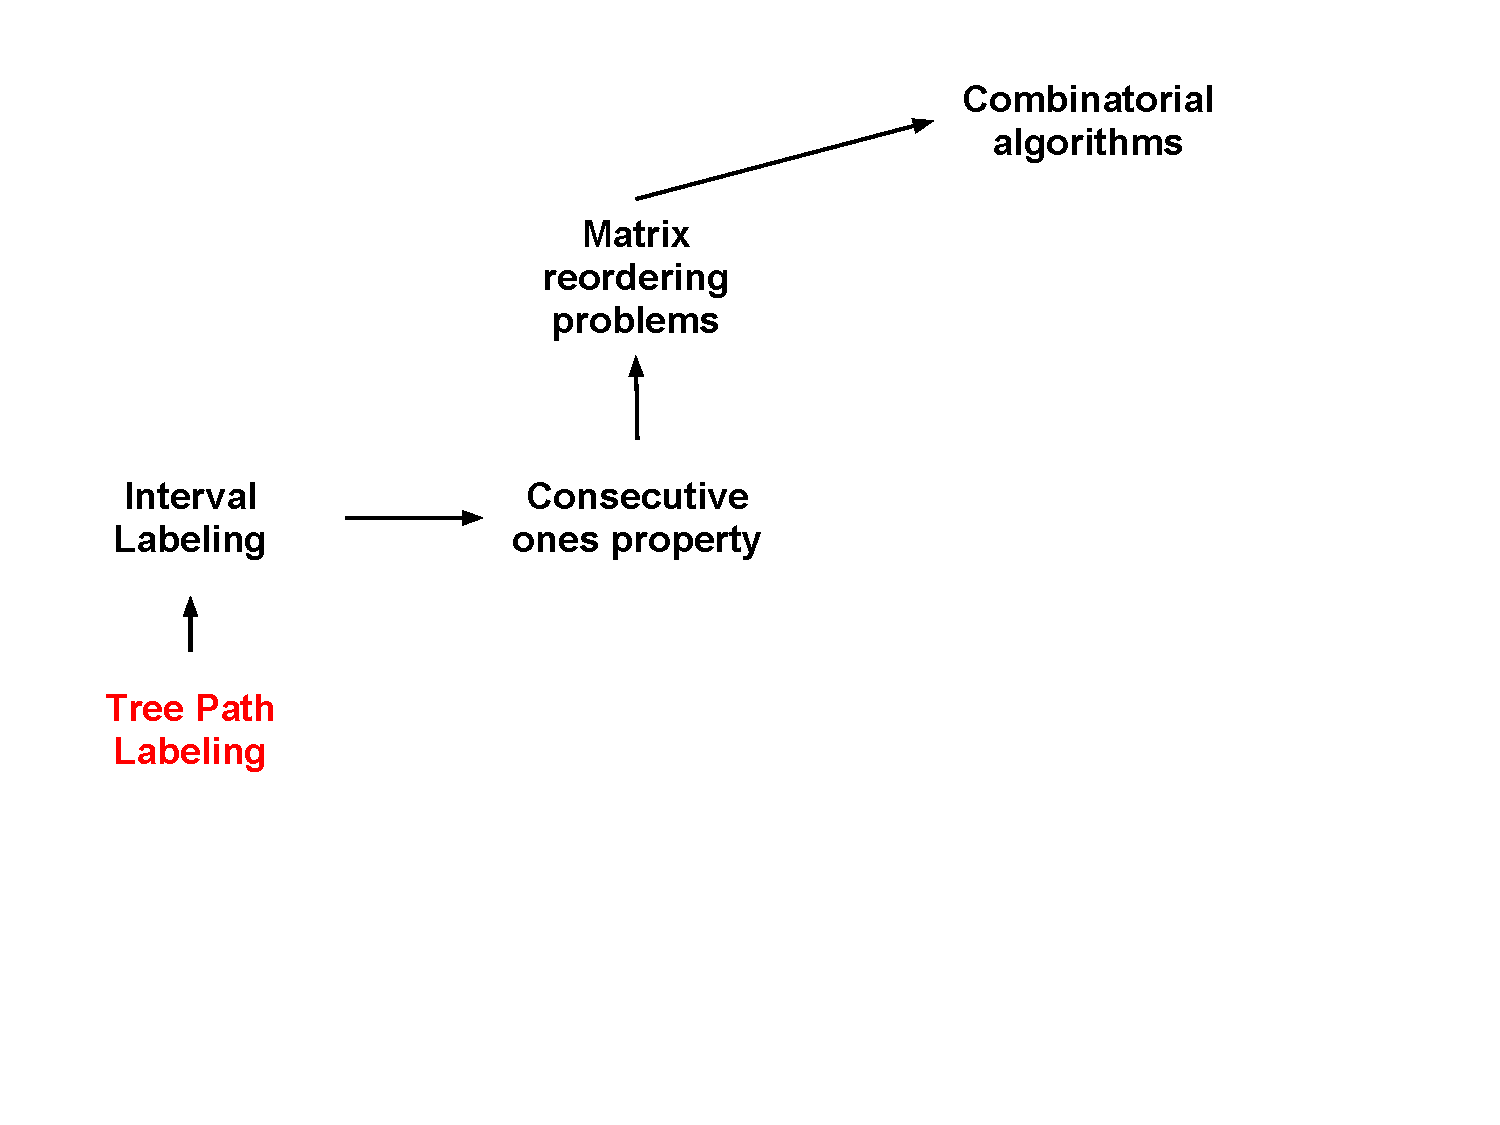
\includegraphics[scale=0.3]{m1.pdf}} 
   \only<2>{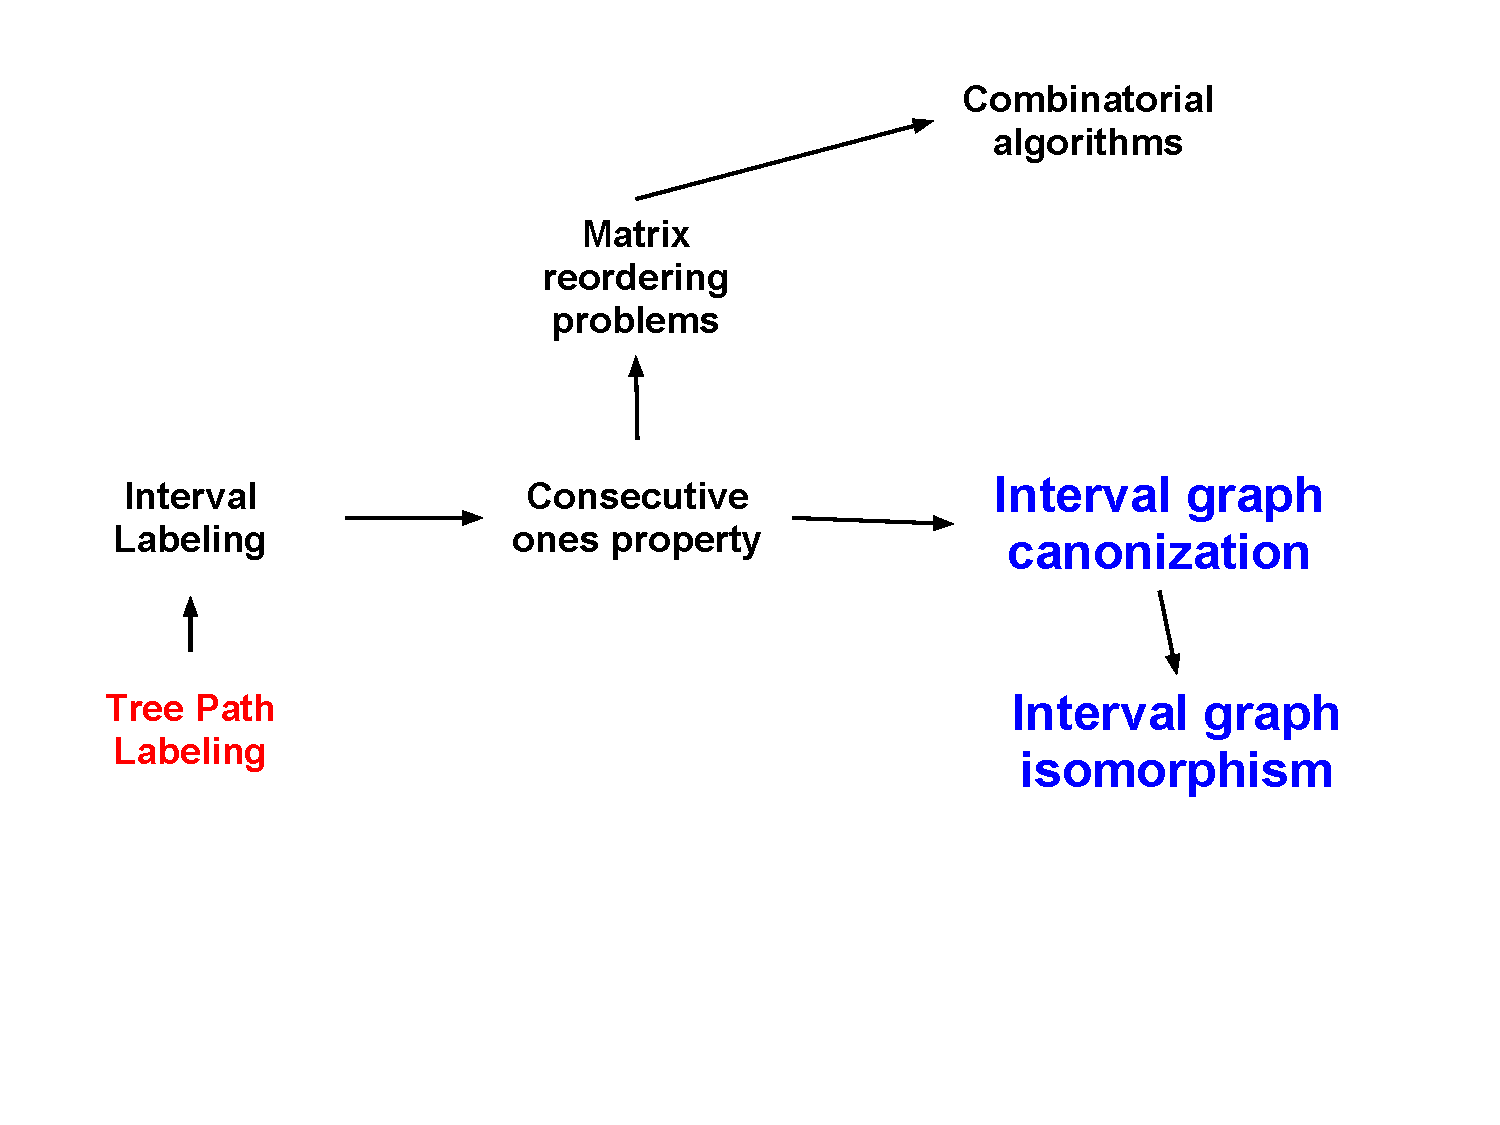
\includegraphics[scale=0.3]{m2.pdf}} 
   \only<3>{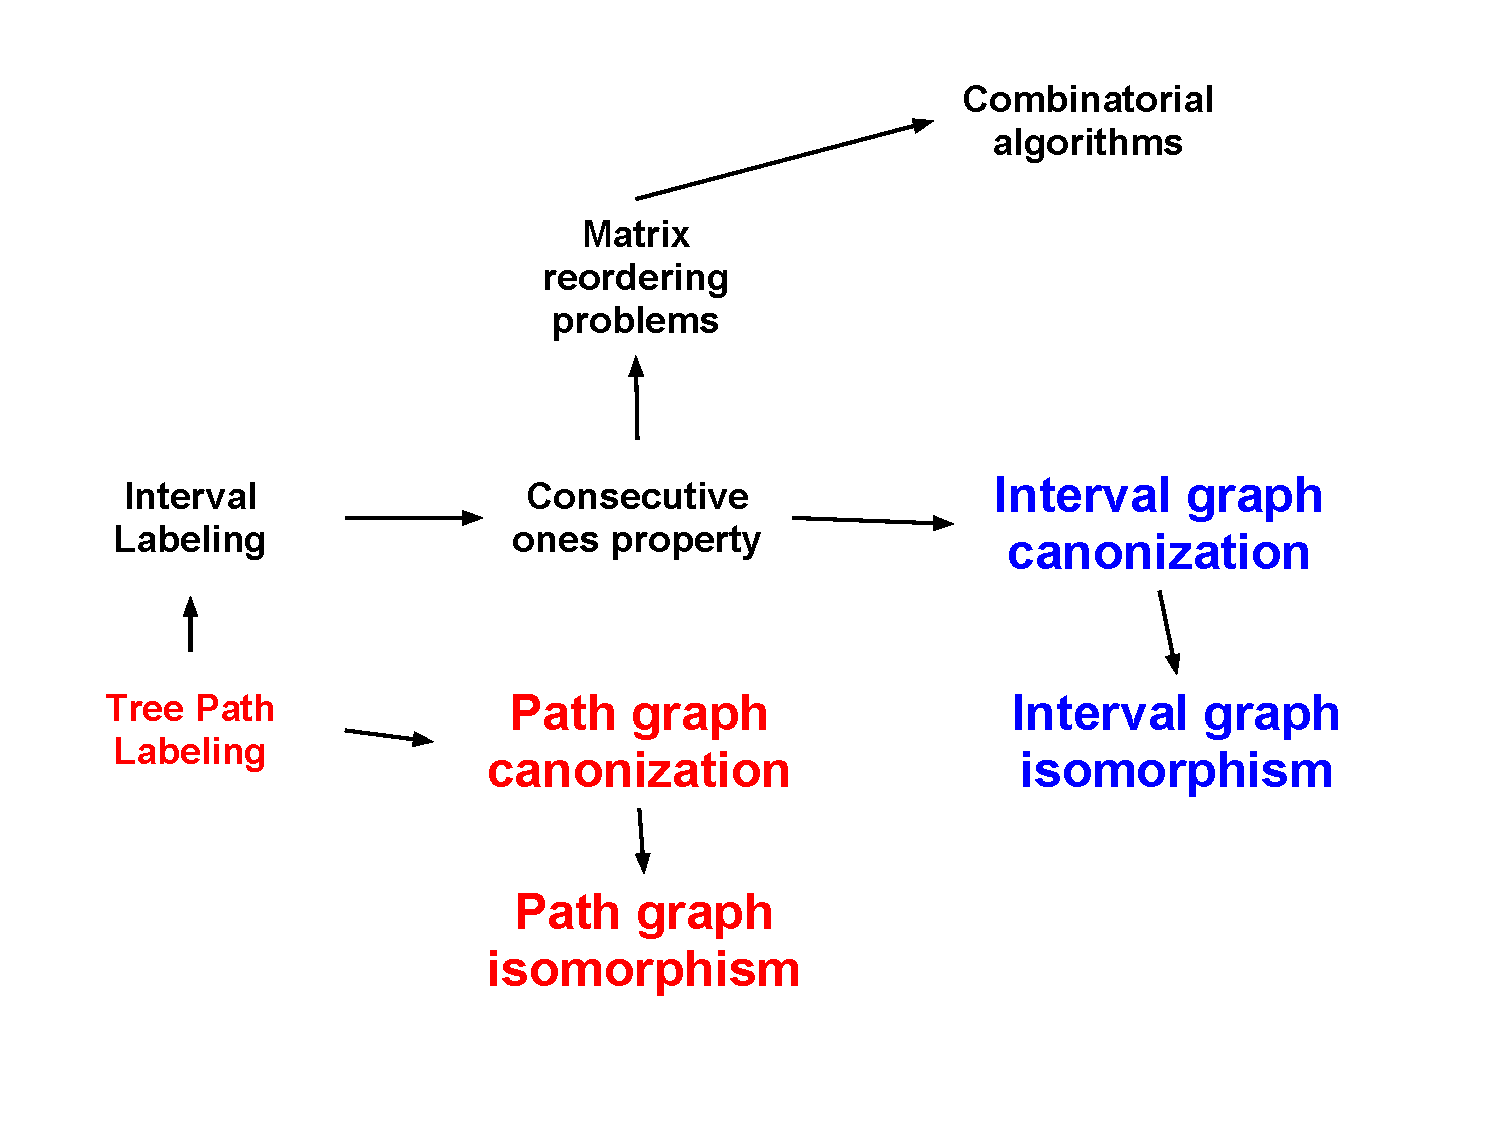
\includegraphics[scale=0.3]{m3.pdf}} 

 \note{}
}

\subsection*{References}
\begin{frame}[allowframebreaks]{References}% {The foundation}
\scriptsize  %\footnotesize
\bibliographystyle{alpha}
\bibliography{./lib/cop-variants_beamer}

\end{frame}

% \begin{frame}
% \end{frame} % TEMP: to enforce toc entries when frames haven't been decided
%             % yet.

\end{document}
